% DOM, Javascript XML, XSL
% capitolo 7 testo e automa di ciotti
% SLIDE Chiara sui fogli di stile
% Capitolo DOM professional Web Dev e XML processing
%

\documentclass{beamer}
    
    %    \usepackage[english]{babel}
        %\usepackage[latin1]{inputenc}
        %\usepackage[T1]{fontenc}
    
    \mode<presentation>{
      \setbeamertemplate{background canvas}[vertical shading]
      \usetheme{Berkeley}
      \useoutertheme{himinfolines}
    }
      
    \usepackage{ucs}
    \usepackage[utf8]{inputenc}
    \usepackage[english,polutonikogreek,italian,UKenglish,british]{babel}
    \usepackage{graphicx}
    \usepackage{colortbl}
    \usepackage{multicol}
    \usepackage{ulem}
    \usepackage{verbatim}
    \usepackage{alltt}
    \usepackage{ccicons}
    \usepackage{MnSymbol,wasysym}
    \usepackage{tikzsymbols}
    \usepackage{textcomp}
    \usepackage{xmpincl}
    
    \usepackage{parskip}
    \setcounter{nframes}{120}
    \setcounter{nframe}{1}
    \setbeamercovered{dynamic}
    \newenvironment{grcenv}{\begin{otherlanguage}{greek}}{\end{otherlanguage}}
    \newcommand{\g}[1]{\textgreek{#1}}
    \definecolor{darkgreen}{rgb}{0,0.5,0}
    \definecolor{darkblue}{rgb}{0,0,0.5}
    \definecolor{grey}{rgb}{0.5,0.5,0.5}
    \setcounter{tocdepth}{5}
    
    \makeatletter
    
    \makeatother
    %\includexmp{LicencesAndLicensing}
    
    %frame00 metadata
        \title{Codifica TEI - Visualizzazione ed Elaborazione: Fogli di Stile}
        \author[A.M. Del Grosso]{Angelo Mario Del Grosso \\ \tiny\textit{(Materiale tratto dalle lezioni di C. Di Pietro)}}
        \institute{\texttt{angelo.delgrosso@ilc.cnr.it} \\\textit{CNR-ILC-LicoLab} \\\url{http://licolab.ilc.cnr.it/}}
        \date{Istituto di Linguistica Computazionale ``A. Zampolli'', \today}
        \AtBeginSection[]{
        \begin{frame}<beamer>
        \addtocounter{nframe}{1}
        \footnotesize
        \frametitle{Progress status}
        \tableofcontents[currentsection,hideothersubsections]
        \end{frame}
        }
    
    \begin{document}
    
    \begin{frame}
        \maketitle
    \end{frame}
    
    \begin{frame}
        \frametitle{Sommario della Lezione}
        \tableofcontents
    \end{frame}
    
    \section{Introduzione ai Fogli di Stile}
    
    \begin{frame}
        \frametitle{Visualizzare ed Elaborare documenti XML}
        \addtocounter{nframe}{1}
        
        %\begin{center}
        %    
\includegraphics[width=.2\textwidth]{../imgs/tei-r.pdf}
        %\end{center}
        %\textit{In parte già disponibili nei moduli TEI di base}

         \begin{block}{Perché visualizzare il testo}
        %     \emph{Per la critica testuale indispensabili i moduli}
             \begin{itemize}
                \item Controllare la codifica e correggere i refusi
                \item Assicurarsi che tutto sia stato trascritto correttamente
                \item Mostrare il testo a persone che non conoscono XML-TEI
                \item Disporre di una versione del lavoro fruibile
            \end{itemize}
         \end{block}
        
    \end{frame}
    
    \begin{frame}
        \frametitle{Visualizzare ed Elaborare documenti XML}
        \addtocounter{nframe}{1}
        
        \begin{block}{I fogli di stile (style sheet)}
           \begin{itemize}
               \item Descrive il modo in cui un documento elettronico deve essere visualizzato
               \item Il mezzo di visualizzazione può variare: lo schermo di un computer, la stampa, i sintetizzatori vocali, ecc.
           \end{itemize}
        \end{block}
        
    \end{frame}
    
    \begin{frame}
        \frametitle{Visualizzare ed Elaborare documenti XML}
        \addtocounter{nframe}{1}
        
        \begin{block}{Scopo dei fogli di stile}
           \begin{itemize}
               \item \emph{Separazione forma-contenuto}: \textit{la visualizzazione del documento è un processo indipendente (e successivo)}
               \item \emph{Gestione della resa grafica} per molti documenti contemporaneamente: \textit{massima uniformità dello stile}
               \item \emph{Gestione di mezzi diversi} dal monitor: smartphone, sintetizzatore
               vocale, stampante braille, ecc.
           \end{itemize}
        \end{block}
        
    \end{frame}

    \begin{frame}
        \frametitle{Visualizzare ed Elaborare documenti XML}
        \addtocounter{nframe}{1}
        
        \begin{block}{Metodi e Tecnologie}
            \textbf{Quelli più noti e utilizzati sono standard internazionali definiti dal consorzio W3 \url{(http://www.w3.org/Style/CSS)}.}
           \begin{itemize}
            \item CSS: Cascading Style Sheets
            \item XSL: eXtensible Stylesheet Language
           \end{itemize}
        \end{block}
        
    \end{frame}

    \begin{frame}
        \frametitle{Visualizzare ed Elaborare documenti XML}
        \addtocounter{nframe}{1}
        
        \begin{block}{CSS: Cascading Style Sheets}
           
           \begin{itemize}
               \item Nati per HTML, possono essere utilizzati anche con XML
               \item Mostrano cosa c'è nel file, nell'ordine in cui questo compare
               \item Molto semplici, ma anche limitati
           \end{itemize}
        \end{block}
        
    \end{frame}

    \begin{frame}
        \frametitle{Visualizzare ed Elaborare documenti XML}
        \addtocounter{nframe}{1}
        
        \begin{block}{XSL: eXtensible Stylesheet Language}
           
           \begin{itemize}
               \item Trasforma XML in qualcos'altro: HTML, PDF, ODT, EPUB
               \item Molto potente, ma complesso e difficile da imparare
           \end{itemize}
        \end{block}
        
    \end{frame}


    \begin{frame}
        \frametitle{Visualizzare ed Elaborare documenti XML}
        \addtocounter{nframe}{1}
        
        \begin{block}{Perché due tipologie di fogli di stile}
           
           \begin{itemize}
               \item I documenti XML possono essere resi in tre modi diversi
               \item Usare CSS quando si può e XSL quando è necessario
           \end{itemize}
        \end{block}
        
    \end{frame}


    \begin{frame}
        \frametitle{Visualizzare ed Elaborare documenti XML}
        \addtocounter{nframe}{1}
        
        \begin{center}
            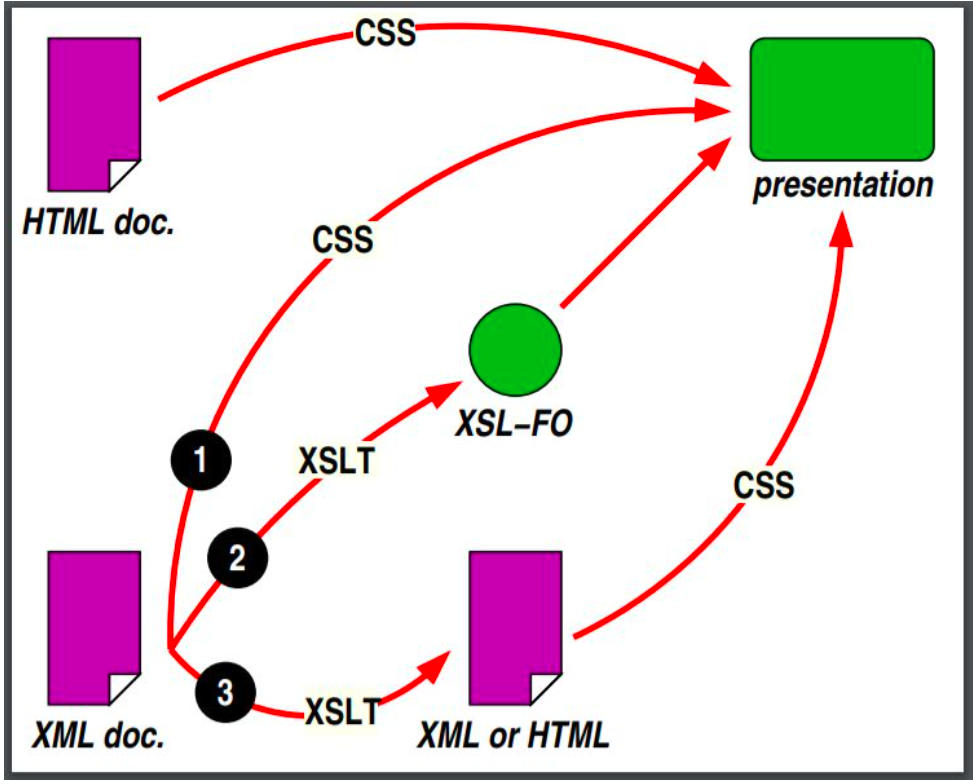
\includegraphics[width=.9\textwidth]{imgs/XML-VisualModality.png}
        \end{center}
        %\textit{In parte già disponibili nei moduli TEI di base}
    
    \end{frame}


    \begin{frame}
        \frametitle{Visualizzare ed Elaborare documenti XML}
        \addtocounter{nframe}{1}
        \begin{center}
            \textbf{CSS e XSL: caratteristiche a confronto}
        \end{center}
       
        \begin{center}
            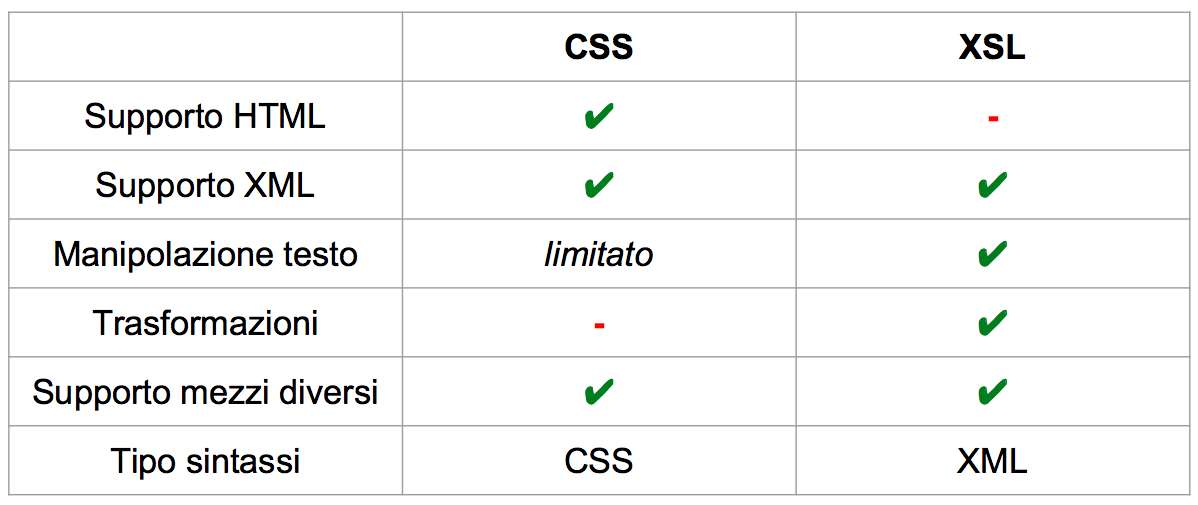
\includegraphics[width=.9\textwidth]{imgs/css-xsl.png}
        \end{center}
        %\textit{In parte già disponibili nei moduli TEI di base}
    
    \end{frame}

    \begin{frame}
        \frametitle{Visualizzare ed Elaborare documenti XML}
        \addtocounter{nframe}{1}
        
        \begin{block}{Fogli di Stile CSS}
           
           \begin{itemize}
               \item Il formato CSS (Cascading Style Sheets) è nato per essere applicato alle pagine HTML.
               \item Ottenere una separazione tra contenuto e forma
               \item Le specifiche dei fogli di stile CSS sono disponibili sul sito \url{http://www.w3.org/Style/CSS}
           \end{itemize}
        \end{block}
        
    \end{frame}

    \begin{frame}
        \frametitle{Visualizzare ed Elaborare documenti XML}
        \addtocounter{nframe}{1}
        
        \begin{block}{Fogli di Stile CSS}
           
           \begin{itemize}
               \item Al momento è in corso di definizione la successiva versione CSS4
               \item La situazione è in costante miglioramento grazie alla nuova generazione
               di navigatori (Firefox, Opera, Konqueror, Safari, Chrome, ecc.)
               \item Possono essere utilizzate anche per documenti XML
           \end{itemize}
        \end{block}
        
    \end{frame}


    \begin{frame}
        \frametitle{Visualizzare ed Elaborare documenti XML}
        \addtocounter{nframe}{1}
        
        \begin{block}{Fogli di Stile CSS}
           
           \begin{itemize}
               \item Offrono limitatissimi mezzi per modificare il documento al quale vengono applicati (in particolare aggiungere testo)
               \item Sono basati su una sintassi specifica piuttosto semplice
           \end{itemize}
        \end{block}
        
    \end{frame}


    \begin{frame}
        \frametitle{Visualizzare ed Elaborare documenti XML}
        \addtocounter{nframe}{1}
        \begin{center}
            \textbf{Sintassi CSS}
        \end{center}
       
        \begin{center}
            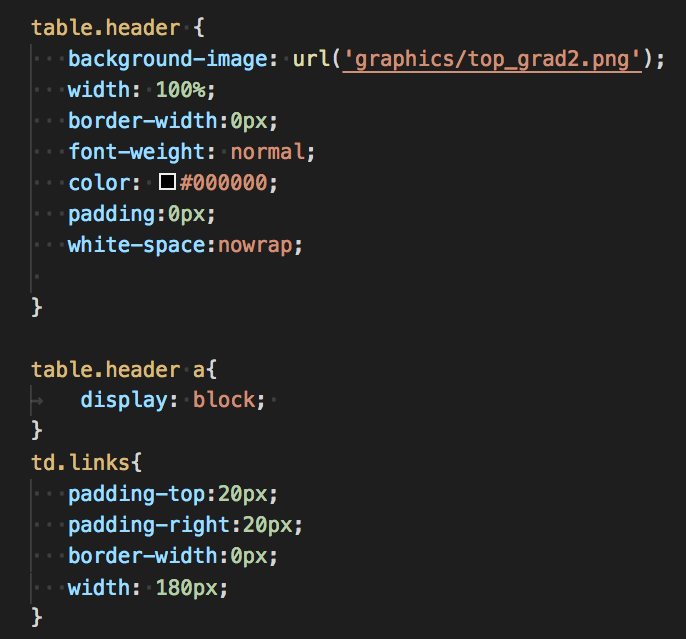
\includegraphics[width=.8\textwidth]{imgs/css-sintassi.png}
        \end{center}
        %\textit{In parte già disponibili nei moduli TEI di base}
    
    \end{frame}

    \begin{frame}
        \frametitle{Visualizzare ed Elaborare documenti XML}
        \addtocounter{nframe}{1}
        \begin{block}{Fogli di Stile CSS: invocazione}
            
            \begin{itemize}
                \item usando \textbf{l’elemento} \texttt{<style>} nel gruppo \texttt{<head>} di un documento HTML/XHTML
                \item con un \textbf{collegamento} all’interno del gruppo \texttt{<head>} di un documento HTML/XHTML
                \item con una \textbf{istruzione} specifica all’inizio di un documento XML
            \end{itemize}
         \end{block}
    
    \end{frame}

    \begin{frame}
        \frametitle{Visualizzare ed Elaborare documenti XML}
        \addtocounter{nframe}{1}
        \begin{block}{Fogli di Stile CSS: invocazione HTML}

            \texttt{<link rel="stylesheet" }
                \\\texttt{ type="text/css" href="default.css" media="screen" > }

         \end{block}

         \begin{block}{Fogli di Stile CSS: invocazione XML}
            
            \texttt{<?xml-stylesheet} 
                \\\texttt{type="text/css" href="style.css"?>}

         \end{block}
    
    \end{frame}

    % \begin{frame}
    %     \frametitle{Modularità della TEI}
    %     \addtocounter{nframe}{1}
        
    %    % \begin{center}
    %     % 
\includegraphics[width=.2\textwidth]{../imgs/tei-r.pdf}
    %     % \end{center}
    
    %     \begin{itemize}
            
    %         \item<1-> parleremo del sistema Modulare della TEI
    %             \begin{itemize}
    %                 \item<1-> Moduli
    %                 \item<1-> Classi
    %                 \item<1-> Macro
    %                 \item<1-> Datatype
    %             \end{itemize} 
    %         \item<2-> parleremo degli elementi basilari
    %             \begin{itemize}
    %                 \item<2-> Intestazione TEI (TEIHeader)
    %                 \item<2-> Elementi e attributi presenti in tutti i documenti TEI
    %                 \item<2-> Esempi di codifica
    %             \end{itemize} 
    %     \end{itemize}
        
    % \end{frame}
    
    \section{XSL Transformations: Caratteristiche Fondamentali}
    \begin{frame}
    \frametitle{Visualizzare ed Elaborare documenti XML}
    \addtocounter{nframe}{1}
    
    %\begin{center}
    %    
\includegraphics[width=.2\textwidth]{../imgs/tei-r.pdf}
    %\end{center}
    %\textit{In parte già disponibili nei moduli TEI di base}

     \begin{block}{Perché visualizzare il testo}
    %     \emph{Per la critica testuale indispensabili i moduli}
         \begin{itemize}
            \item  Controllare la codifica e correggere i refusi
             \item Assicurarsi che tutto sia stato trascritto correttamente
             \item Mostrare il testo a persone che non conoscono XML-TEI
             \item Disporre di una versione del lavoro fuibile
        \end{itemize}
     \end{block}
    
\end{frame}



\begin{frame}
    \frametitle{Fondamenti Extensible Stylesheet Language}
    \addtocounter{nframe}{1}
    
    %\begin{center}
    %    
\includegraphics[width=.2\textwidth]{../imgs/tei-r.pdf}
    %\end{center}
    %\textit{In parte già disponibili nei moduli TEI di base}

     \begin{block}{eXtensible Stylesheet Language (XSL)}
    %     \emph{Per la critica testuale indispensabili i moduli}
         \begin{itemize}
            \item  Specifica del W3C che descrive un metodo per la visualizzazione e manipolazione dei documenti XML.
             \item Maggiore controllo sulla presentazione dei dati XML
             \item Generazione di layout complessi e composti
        \end{itemize}
     \end{block}
    
\end{frame}


\begin{frame}
    \frametitle{Fondamenti Extensible Stylesheet Language}
    \addtocounter{nframe}{1}
    
    %\begin{center}
    %    
\includegraphics[width=.2\textwidth]{../imgs/tei-r.pdf}
    %\end{center}
    %\textit{In parte già disponibili nei moduli TEI di base}

     \begin{block}{XSL incorpora tre linguaggi}
    %     \emph{Per la critica testuale indispensabili i moduli}
         \begin{itemize}
            \item \textbf{XSL Transformations (XSL-T)}: \textit{trasformazione di un documento XML in un altro tipo di documento} (es.: HTML)
            \item \textbf{XSL Formatting Objects (XSL-FO)}: \textit{applicazione degli stili e della resa grafica di un documento XML}
            \item \textbf{XML Path (XPath)}: \textit{usato nei fogli di stile XSLT per selezionare le parti di un documento XML}
        \end{itemize}
     \end{block}
    
\end{frame}

\begin{frame}
    \frametitle{Fondamenti Extensible Stylesheet Language}
    \addtocounter{nframe}{1}
    
    \begin{center}
        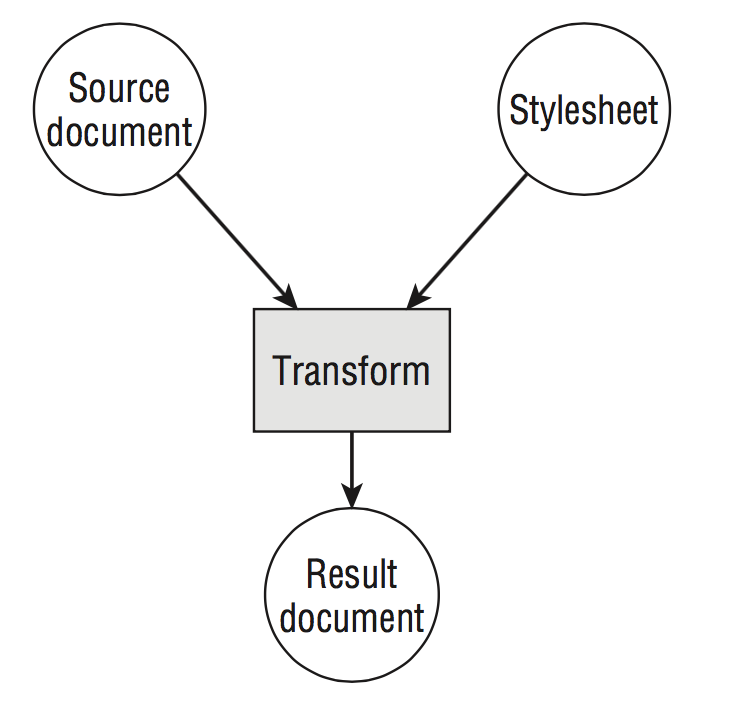
\includegraphics[width=.8\textwidth]{imgs/SchemaXSLTprocessing.png}
    \end{center}
    %\textit{In parte già disponibili nei moduli TEI di base}

\end{frame}

\begin{frame}
    \frametitle{Fondamenti Extensible Stylesheet Language}
    \addtocounter{nframe}{1}
    
    %\begin{center}
    %    
\includegraphics[width=.2\textwidth]{../imgs/tei-r.pdf}
    %\end{center}
    %\textit{In parte già disponibili nei moduli TEI di base}

     \begin{block}{XSL Transformations}
    %     \emph{Per la critica testuale indispensabili i moduli}
         \begin{itemize}
            \item XSLT è un vero e proprio linguaggio di programmazione che usa la sintassi XML
            \item Usa namespace differenti per distinguere fra istruzioni proprie (precedute da \textbf{xsl:}) e output
            \item Legge e scrive alberi XML (ma è possibile ottenere come output anche del
            codice HTML o del testo semplice)
            \item Versione attuale: XSLT 3.0 \url{(https://www.w3.org/TR/xslt-30/)}
        \end{itemize}
     \end{block}
    
\end{frame}

\begin{frame}
    \frametitle{Fondamenti Extensible Stylesheet Language}
    \addtocounter{nframe}{1}
    
    %\begin{center}
    %    
\includegraphics[width=.2\textwidth]{../imgs/tei-r.pdf}
    %\end{center}
    %\textit{In parte già disponibili nei moduli TEI di base}

     \begin{block}{XSL Capacità di trasformazione}
    %     \emph{Per la critica testuale indispensabili i moduli}
         \begin{itemize}
            \item generazione di testo costante;
            \item soppressione del contenuto;
            \item spostamento del testo (es., scambio ordine di nome e cognome);
            \item duplicazione del testo (ad es., tabella di contenuti copiando i titoli);
            \item ordinamento dei contenuti (ad es, termini in ordine alfabetico);
            \item elaborazione di nuove informazioni in base a quelle esistenti (es. statistiche)
        \end{itemize}
     \end{block}
    
\end{frame}

\begin{frame}
    \frametitle{Fondamenti Extensible Stylesheet Language}
    \addtocounter{nframe}{1}
    
    %\begin{center}
    %    
\includegraphics[width=.2\textwidth]{../imgs/tei-r.pdf}
    %\end{center}
    %\textit{In parte già disponibili nei moduli TEI di base}

     \begin{block}{Caratteristiche fondamentali di XSLT}
    %     \emph{Per la critica testuale indispensabili i moduli}
         \begin{itemize}
            \item Basato su regole di trasformazione (\textit{modello pattern-match})
            \item Le regole sono dichiarative \textit{(specificano che cosa deve essere generato quando si incontra un certo modello nel documento)}
            \item Le regole possono essere disposte in qualsiasi ordine
        \end{itemize}
     \end{block}
    
\end{frame}


\begin{frame}
    \frametitle{Fondamenti Extensible Stylesheet Language}
    \addtocounter{nframe}{1}
    
    %\begin{center}
    %    
\includegraphics[width=.2\textwidth]{../imgs/tei-r.pdf}
    %\end{center}
    %\textit{In parte già disponibili nei moduli TEI di base}

     \begin{block}{Modalità di Trasformazioni XSLT}
    %     \emph{Per la critica testuale indispensabili i moduli}
         \begin{itemize}
            \item \textbf{Lato server}, utilizzando script Java, ASP, PHP etc. , per produrre “al volo” pagine HTML sulla base di documenti XML (es. Cocoon);
            \item \textbf{Lato client}, sui Browser che supportano questa tecnologia;
            \item tramite un programma separato (come ad esempio Oxygen), che permette di applicare uno o più scenari di trasformazione.
        \end{itemize}
     \end{block}
    
\end{frame}

\begin{frame}
    \frametitle{Fondamenti Extensible Stylesheet Language}
    \addtocounter{nframe}{1}
    
    %\begin{center}
    %    
\includegraphics[width=.2\textwidth]{../imgs/tei-r.pdf}
    %\end{center}
    %\textit{In parte già disponibili nei moduli TEI di base}

     \begin{block}{Componenti di Base di un foglio XSLT}
    %     \emph{Per la critica testuale indispensabili i moduli}
         \begin{itemize}
            \item Intestazione XML
            \item Elemento radice \textit{stylesheet} e namespace
            \item Eventuali istruzioni di elaborazione
            \item Serie di template rules
        \end{itemize}
     \end{block}
    
\end{frame}

\begin{frame}
    \frametitle{Fondamenti Extensible Stylesheet Language}
    \addtocounter{nframe}{1}
    
    %\begin{center}
    %    
\includegraphics[width=.2\textwidth]{../imgs/tei-r.pdf}
    %\end{center}
    %\textit{In parte già disponibili nei moduli TEI di base}

     \begin{block}{Intestazione XML}
        \texttt{<?xml version="1.0" encoding="UTF-8" ?>}
     \end{block}

     \begin{block}{Elemento radice}
        \texttt{<xsl:stylesheet version='2.0'}
            \\\texttt{  xmlns:xsl='http://www.w3.org/1999/XSL/Transform'>}
     \end{block}
    
\end{frame}

\begin{frame}
    \frametitle{Fondamenti Extensible Stylesheet Language}
    \addtocounter{nframe}{1}
    
    %\begin{center}
    %    
\includegraphics[width=.2\textwidth]{../imgs/tei-r.pdf}
    %\end{center}
    %\textit{In parte già disponibili nei moduli TEI di base}

     \begin{block}{Eventuali istruzioni di elaborazione}
        \texttt{<xsl:output method="xml" version="1.0" indent="yes"/>}
     \end{block}

     \begin{block}{Serie di template rules}
        \texttt{<xsl:template match="/" > ...</xsl:template>} 
        \\\texttt{<xsl:template match="title" > ... </xsl:template>}
     \end{block}
    
\end{frame}

\begin{frame}
    \frametitle{Fondamenti Extensible Stylesheet Language}
    \addtocounter{nframe}{1}
    
    \begin{center}
        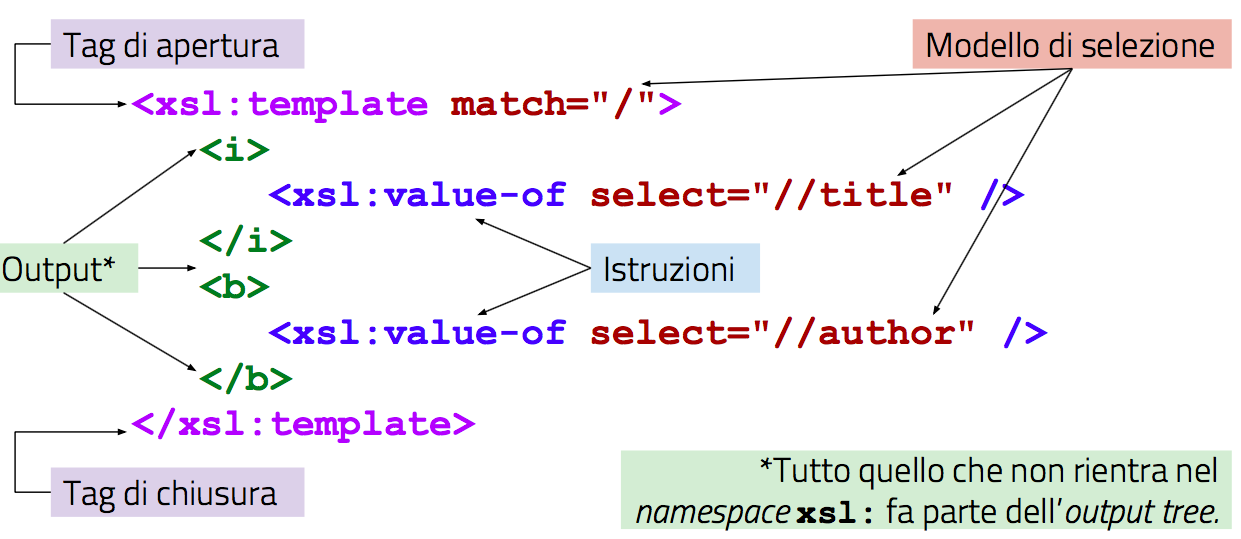
\includegraphics[width=.8\textwidth]{imgs/template-modello.png}
    \end{center}
    %\textit{In parte già disponibili nei moduli TEI di base}

\end{frame}

\begin{frame}
    \frametitle{Fondamenti Extensible Stylesheet Language}
    \addtocounter{nframe}{1}
    
    %\begin{center}
    %    
\includegraphics[width=.2\textwidth]{../imgs/tei-r.pdf}
    %\end{center}
    %\textit{In parte già disponibili nei moduli TEI di base}

     \begin{block}{Come vengono applicate le regole XSLT}
        \emph{Il processore XSLT}
         \begin{itemize}
            \item Legge il documento XML in input e crea l’albero corrispondente
            \item Inizia a percorrere l’albero leggendo i singoli nodi
            \item Confronta Ogni nodo con le regole presenti nel foglio di stile
            \item Produce l’output secondo le istruzioni della regola
            \item Restituisce un albero di output
        \end{itemize}
     \end{block}
    
\end{frame}

\begin{frame}
    \frametitle{Fondamenti Extensible Stylesheet Language}
    \addtocounter{nframe}{1}
    
    \begin{center}
        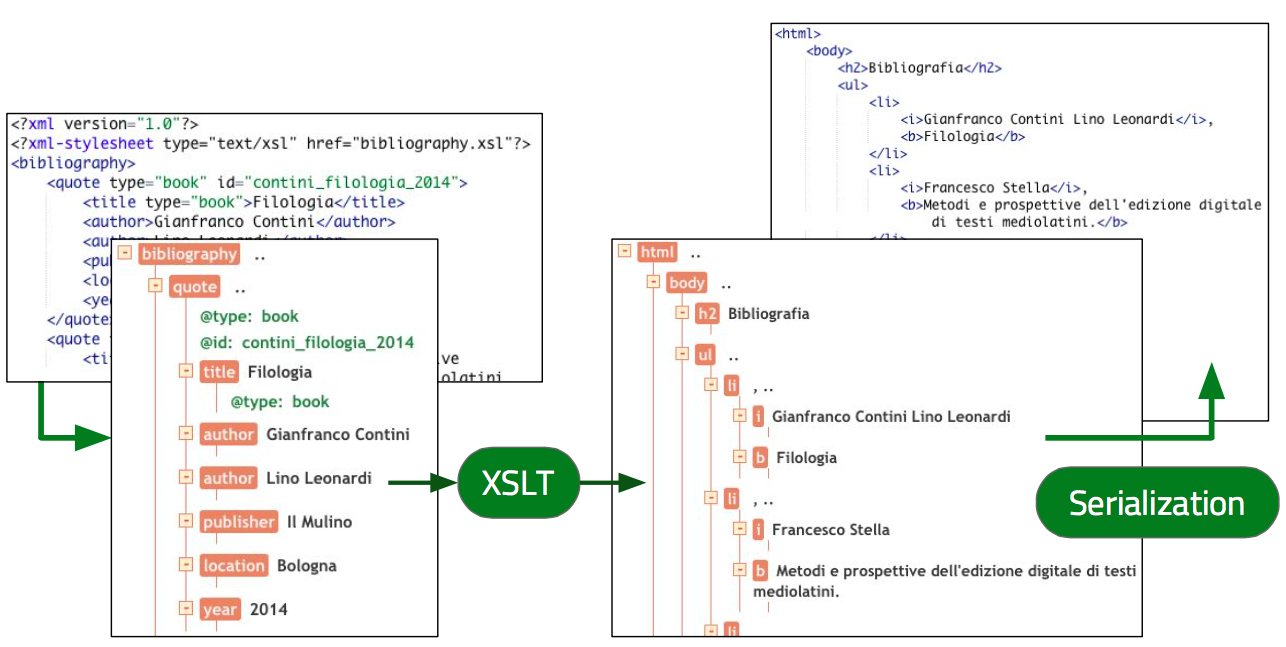
\includegraphics[width=.8\textwidth]{imgs/Processo-xslt.png}
    \end{center}
    %\textit{In parte già disponibili nei moduli TEI di base}

\end{frame}


\begin{frame}
    \frametitle{Fondamenti Extensible Stylesheet Language}
    \addtocounter{nframe}{1}
    
    %\begin{center}
    %    
\includegraphics[width=.2\textwidth]{../imgs/tei-r.pdf}
    %\end{center}
    %\textit{In parte già disponibili nei moduli TEI di base}

     \begin{block}{Esempio di trasformazione}
         Nella sotto-cartella xsl della cartella src leggere il file d'esercizio e individuare le varie componenti.
     \end{block}
    
\end{frame}

\begin{frame}
    \frametitle{Fondamenti Extensible Stylesheet Language}
    \addtocounter{nframe}{1}
    
    %\begin{center}
    %    
\includegraphics[width=.2\textwidth]{../imgs/tei-r.pdf}
    %\end{center}
    %\textit{In parte già disponibili nei moduli TEI di base}

     \begin{block}{Tipi di nodo nell'albero XML}
         \begin{itemize}
            \item \textbf{Radice} del Documento
            \item \textbf{Elementi} con contentuto del sotto albero
            \item \textbf{Attributi}
            \item \textbf{Testo} compresi gli spazi vuoti
            \item \textbf{Commenti} (contenuto tra \texttt{<!-- -->})
            \item \textbf{Namespace} con riferimenti e URI
            \item \textbf{Istruzioni di elaborazione} (contenuto tra \texttt{<? ?>})
        \end{itemize}
     \end{block}
    
\end{frame}

\begin{frame}
    \frametitle{Fondamenti Extensible Stylesheet Language}
    \addtocounter{nframe}{1}
    
    %\begin{center}
    %    
\includegraphics[width=.2\textwidth]{../imgs/tei-r.pdf}
    %\end{center}
    %\textit{In parte già disponibili nei moduli TEI di base}

     \begin{block}{Tipi di nodo nell'albero XML}
         \begin{itemize}
            \item Il \textbf{documento} stesso costituisce la radice (\textit{l’elemento radice XML non è la radice dell'albero di rappresentazione!})
            \item L'intero albero è suddivisibile in sotto-alberi
            \item I nodi più importanti sono gli elementi e i loro attributi
            \item Le entità vengono "tradotte" nel testo loro assegnato al momento
            della dichiarazione
            \item Lo spazio "vuoto" può essere considerato o no
        \end{itemize}
     \end{block}
    
\end{frame}

\begin{frame}
    \frametitle{Fondamenti Extensible Stylesheet Language}
    \addtocounter{nframe}{1}
    
    \begin{center}
        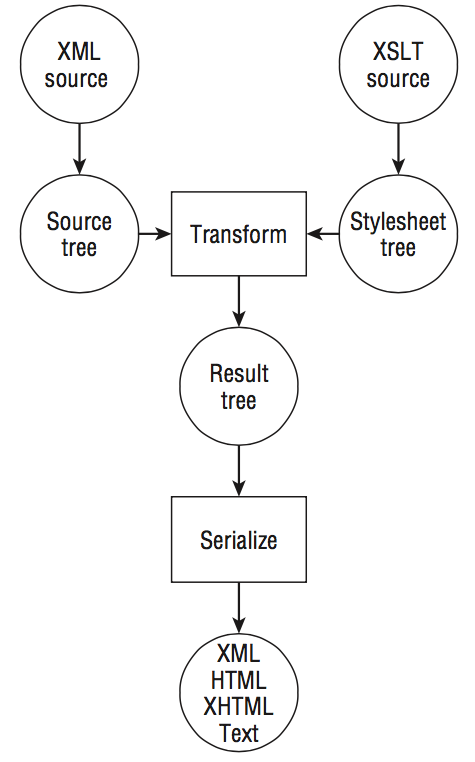
\includegraphics[width=.8\textwidth]{imgs/Schema-trasformazione.png}
    \end{center}
    %\textit{In parte già disponibili nei moduli TEI di base}

\end{frame}


    
    \section{Template (rules/named) e principali istruzioni XSLT}
    \begin{frame}
    \frametitle{Visualizzare ed Elaborare documenti XML}
    \addtocounter{nframe}{1}
    
    %\begin{center}
    %    
\includegraphics[width=.2\textwidth]{../imgs/tei-r.pdf}
    %\end{center}
    %\textit{In parte già disponibili nei moduli TEI di base}

     \begin{block}{Perché visualizzare il testo}
    %     \emph{Per la critica testuale indispensabili i moduli}
         \begin{itemize}
            \item  Controllare la codifica e correggere i refusi
             \item Assicurarsi che tutto sia stato trascritto correttamente
             \item Mostrare il testo a persone che non conoscono XML-TEI
             \item Disporre di una versione del lavoro fuibile
        \end{itemize}
     \end{block}
    
\end{frame}

\begin{frame}
    \frametitle{Visualizzare ed Elaborare documenti XML}
    \addtocounter{nframe}{1}
    
    %\begin{center}
    %    
\includegraphics[width=.2\textwidth]{../imgs/tei-r.pdf}
    %\end{center}
    %\textit{In parte già disponibili nei moduli TEI di base}

     \begin{block}{Elemento \texttt{<xsl:template>}}
        Definisce una regola (ovvero un modello) di trasformazione per i nodi di un particolare tipo/contesto.
     \end{block}
    
\end{frame}

\begin{frame}
    \frametitle{Visualizzare ed Elaborare documenti XML}
    \addtocounter{nframe}{1}
    
    \begin{center}
        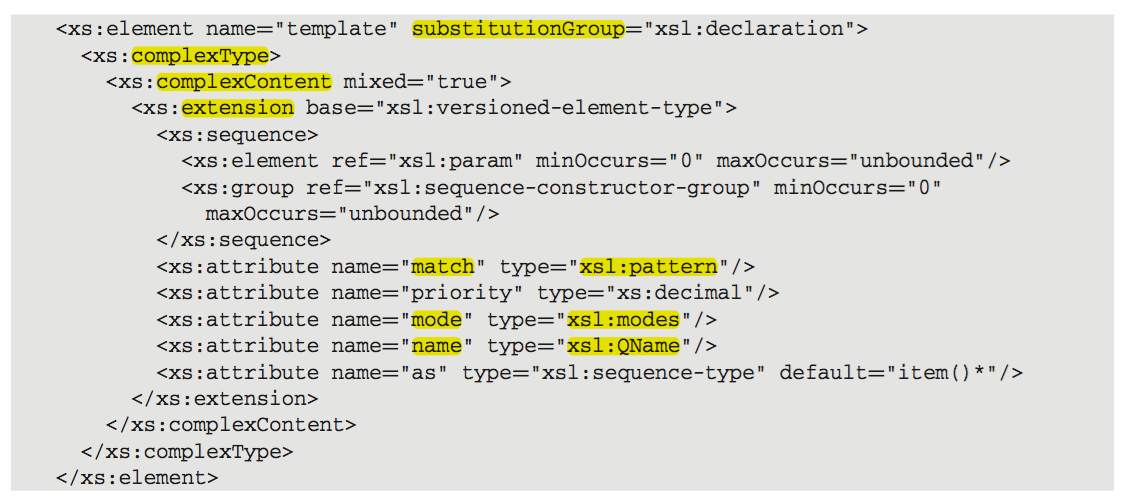
\includegraphics[width=.9\textwidth]{imgs/Schema-template.png}
    \end{center}
    %\textit{In parte già disponibili nei moduli TEI di base}

\end{frame}

\begin{frame}
    \frametitle{Visualizzare ed Elaborare documenti XML}
    \addtocounter{nframe}{1}
    
    %\begin{center}
    %    
\includegraphics[width=.2\textwidth]{../imgs/tei-r.pdf}
    %\end{center}
    %\textit{In parte già disponibili nei moduli TEI di base}

     \begin{block}{Attributi Elemento \texttt{<xsl:template>}}
    %     \emph{Per la critica testuale indispensabili i moduli}
         \begin{itemize}
             \item \textbf{name}: nome del template;
             \item \textbf{match}: pattern che indica l'elemento su cui applicare il modello;
             \item \textbf{priority}: priorità del modello;
             \item \textbf{mode}: modalità di elaborazione, che consente all'elemento di essere elaborato più volte per produrre un risultato diverso ogni volta.
        \end{itemize}
     \end{block}
    
\end{frame}


\begin{frame}
    \frametitle{Visualizzare ed Elaborare documenti XML}
    \addtocounter{nframe}{1}
    
    %\begin{center}
    %    
\includegraphics[width=.2\textwidth]{../imgs/tei-r.pdf}
    %\end{center}
    %\textit{In parte già disponibili nei moduli TEI di base}

     \begin{block}{Elemento \texttt{<xsl:template>}}
        \textit{I template XSLT possono avere due forme: }
        \begin{itemize}
            \item \textbf{"tempate rules"} che specificano una regola con pattern-matching ( \texttt{<xsl:apply-templates>})
            \item \textbf{named templates} che specificano regole che possono essere chiamate esplicitamente con \texttt{<xsl:call-template>}
        \end{itemize}

     \end{block}
    
\end{frame}


%% value-of

\begin{frame}
    \frametitle{Visualizzare ed Elaborare documenti XML}
    \addtocounter{nframe}{1}
    
    %\begin{center}
    %    
\includegraphics[width=.2\textwidth]{../imgs/tei-r.pdf}
    %\end{center}
    %\textit{In parte già disponibili nei moduli TEI di base}

     \begin{block}{Elemento \texttt{<xsl:value-of>}}
        Restituisce il contenuto del nodo selezionato secondo l'espressione XPath indicata.
        \\ \textit{(Il contenuto di un elemento è costituito da tutti i caratteri che si trovano fra tag di apertura e tag di chiusura)}
     \end{block}
    
\end{frame}

\begin{frame}
    \frametitle{Visualizzare ed Elaborare documenti XML}
    \addtocounter{nframe}{1}
    
    \begin{center}
        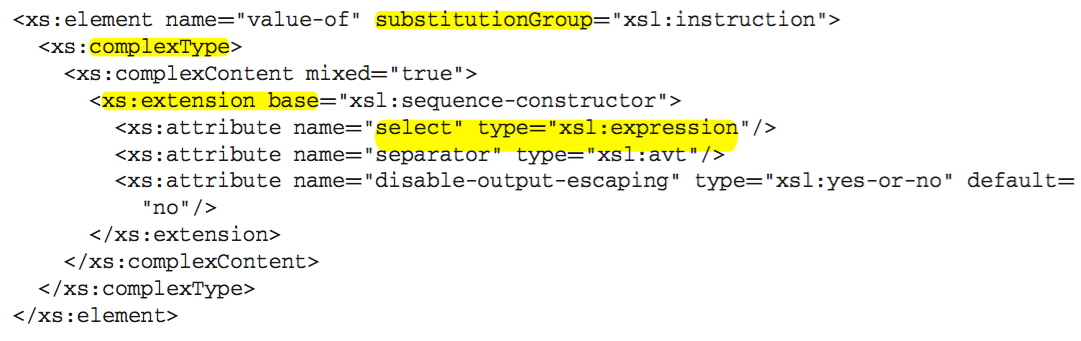
\includegraphics[width=.9\textwidth]{imgs/Schema-value-of.png}
    \end{center}
    %\textit{In parte già disponibili nei moduli TEI di base}

\end{frame}

\begin{frame}
    \frametitle{Visualizzare ed Elaborare documenti XML}
    \addtocounter{nframe}{1}
    
    %\begin{center}
    %    
\includegraphics[width=.2\textwidth]{../imgs/tei-r.pdf}
    %\end{center}
    %\textit{In parte già disponibili nei moduli TEI di base}

     \begin{block}{Attributi Elemento \texttt{<xsl:value-of>}}
    %     \emph{Per la critica testuale indispensabili i moduli}
         \begin{itemize}
             \item \textbf{select}: espressione XPath da valutare nel contesto corrente
             \item \textbf{disable-output-escaping}: default "no"; se "yes", il testo di
             output non esclude i caratteri XML dal testo
        \end{itemize}
     \end{block}
    
\end{frame}

\begin{frame}
    \frametitle{Visualizzare ed Elaborare documenti XML}
    \addtocounter{nframe}{1}
    
    %\begin{center}
    %    
\includegraphics[width=.2\textwidth]{../imgs/tei-r.pdf}
    %\end{center}
    %\textit{In parte già disponibili nei moduli TEI di base}

     \begin{block}{Esempio Elemento \texttt{<xsl:value-of>}}
        
        \texttt{<xsl:template match="fileDesc" >}
        \\\texttt{<h1>File Desc</h1>}
        \\\texttt{<p>}
            \\\texttt{<xsl:value-of select="titleStmt/title" disable-output-escaping="no" />}
        \\\texttt{</p>}
        \\\texttt{</xsl:template>}

     \end{block}
    
\end{frame}

%% Apply-templates

\begin{frame}
    \frametitle{Visualizzare ed Elaborare documenti XML}
    \addtocounter{nframe}{1}
    
    %\begin{center}
    %    
\includegraphics[width=.2\textwidth]{../imgs/tei-r.pdf}
    %\end{center}
    %\textit{In parte già disponibili nei moduli TEI di base}

     \begin{block}{Elemento \texttt{<xsl:apply-templates>}}
        Elaborare in modo ricorsivo i nodi di un documento XML a partire da un punto preciso dell'albero XML.
     \end{block}

     \begin{block}{Elemento \texttt{<xsl:apply-templates>}}
        Confronta ogni nodo presente all’interno del nodo selezionato con le template rules del foglio di stile e se viene trovata una regola applicabile questa viene applicata.
     \end{block}

\end{frame}

\begin{frame}
    \frametitle{Visualizzare ed Elaborare documenti XML}
    \addtocounter{nframe}{1}
    
    \begin{center}
        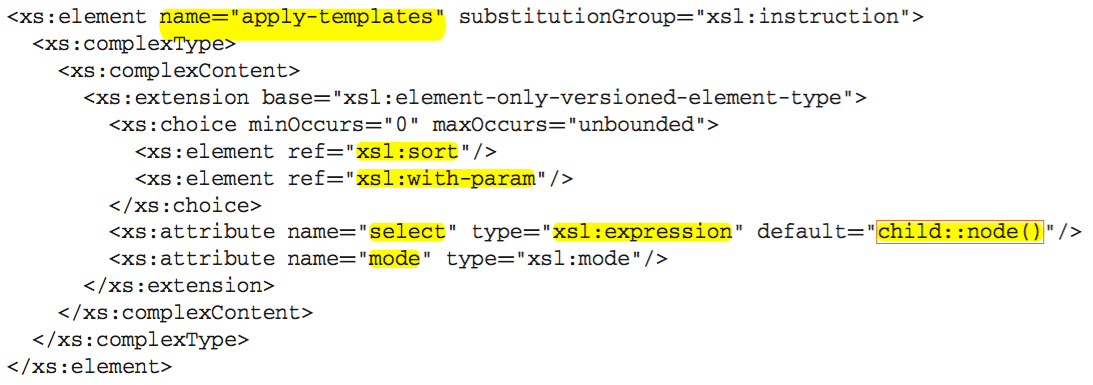
\includegraphics[width=.9\textwidth]{imgs/Schema-apply-templates.png}
    \end{center}
    %\textit{In parte già disponibili nei moduli TEI di base}

\end{frame}

\begin{frame}
    \frametitle{Visualizzare ed Elaborare documenti XML}
    \addtocounter{nframe}{1}
    
    %\begin{center}
    %    
\includegraphics[width=.2\textwidth]{../imgs/tei-r.pdf}
    %\end{center}
    %\textit{In parte già disponibili nei moduli TEI di base}

     \begin{block}{Attributi Elemento \texttt{<xsl:apply-templates>}}
    %     \emph{Per la critica testuale indispensabili i moduli}
         \begin{itemize}
             \item \textbf{select}: espressione XPath
             \item \textbf{mode}: modalità di elaborazione
        \end{itemize}
     \end{block}
    
\end{frame}

\begin{frame}
    \frametitle{Visualizzare ed Elaborare documenti XML}
    \addtocounter{nframe}{1}
    
    %\begin{center}
    %    
\includegraphics[width=.2\textwidth]{../imgs/tei-r.pdf}
    %\end{center}
    %\textit{In parte già disponibili nei moduli TEI di base}

     \begin{block}{Esempio Elemento \texttt{<xsl:apply-templates>}}
        
        \texttt{<xsl:template match="/" >}
        \\\texttt{<html><head>}
        \\\texttt{<title><xsl:value-of select="TEI/teiHeader/fileDesc/title"/></title></head>}
        \\\texttt{<body><div><span>1.</span>}
        \\\texttt{<xsl:apply-templates select="TEI/teiHeader/fileDesc" />}
        \\\texttt{</div></body></html></xsl:template>}

     \end{block}
    
\end{frame}


%% xsl:for-each

\begin{frame}
    \frametitle{Visualizzare ed Elaborare documenti XML}
    \addtocounter{nframe}{1}
    
    %\begin{center}
    %    
\includegraphics[width=.2\textwidth]{../imgs/tei-r.pdf}
    %\end{center}
    %\textit{In parte già disponibili nei moduli TEI di base}

     \begin{block}{Elemento \texttt{<xsl:for-each>}}
        Se sono presenti più nodi con lo stesso nome (e manca un’istruzione ricorsiva precedente) \texttt{<xsl:value-of>} restituisce il valore del primo che incontra.
     \end{block}

     \begin{block}{Elemento \texttt{<xsl:for-each>}}
        È quindi possibile usare l’istruzione \texttt{<xsl:for-each>} e applicare un’istruzione \texttt{<xsl:value-of>} a tutti i nodi identificati dalla regola.
     \end{block}

\end{frame}

\begin{frame}
    \frametitle{Visualizzare ed Elaborare documenti XML}
    \addtocounter{nframe}{1}
    
    \begin{center}
        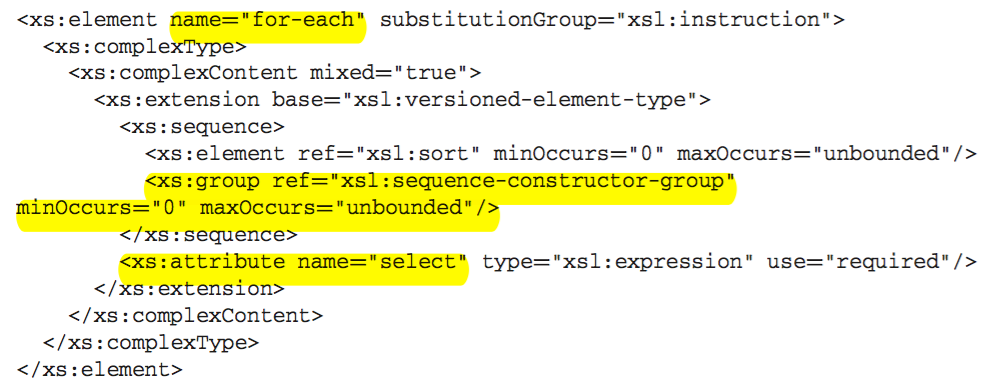
\includegraphics[width=.9\textwidth]{imgs/Schema-for-each.png}
    \end{center}
    %\textit{In parte già disponibili nei moduli TEI di base}

\end{frame}

\begin{frame}
    \frametitle{Visualizzare ed Elaborare documenti XML}
    \addtocounter{nframe}{1}
    
    %\begin{center}
    %    
\includegraphics[width=.2\textwidth]{../imgs/tei-r.pdf}
    %\end{center}
    %\textit{In parte già disponibili nei moduli TEI di base}

     \begin{block}{Attributi Elemento \texttt{<xsl:for-each>}}
    %     \emph{Per la critica testuale indispensabili i moduli}
         \begin{itemize}
             \item \textbf{select}: espressione XPath
        \end{itemize}
     \end{block}
    
\end{frame}

\begin{frame}
    \frametitle{Visualizzare ed Elaborare documenti XML}
    \addtocounter{nframe}{1}
    
    %\begin{center}
    %    
\includegraphics[width=.2\textwidth]{../imgs/tei-r.pdf}
    %\end{center}
    %\textit{In parte già disponibili nei moduli TEI di base}

     \begin{block}{Esempio Elemento \texttt{<xsl:for-each>}}
        
        \texttt{<xsl:template match="/" >}
        \\\texttt{<html><head>}
        \\\texttt{<title><xsl:value-of select="TEI/teiHeader/fileDesc/title"/></title></head>}
        \\\texttt{<body><div>}
        \\\texttt{<xsl:for-each select="//div" >}
        \\\texttt{<div><xsl:value-of select="./p" /></div>}
        \\\texttt{</xsl:for-each></div></body></html>}
     \end{block}
    
\end{frame}


%% xsl:text


\begin{frame}
    \frametitle{Visualizzare ed Elaborare documenti XML}
    \addtocounter{nframe}{1}
    
    %\begin{center}
    %    
\includegraphics[width=.2\textwidth]{../imgs/tei-r.pdf}
    %\end{center}
    %\textit{In parte già disponibili nei moduli TEI di base}

     \begin{block}{Elemento \texttt{<xsl:text>}}
        Permette di inserire una stringa di testo nell’albero di output.
     \end{block}

     \begin{block}{Elemento \texttt{<xsl:text>}}
        Molto utile se si è deciso di eliminare tutti gli spazi e gli a capo.
     \end{block}
     

\end{frame}

\begin{frame}
    \frametitle{Visualizzare ed Elaborare documenti XML}
    \addtocounter{nframe}{1}
    
    \begin{center}
        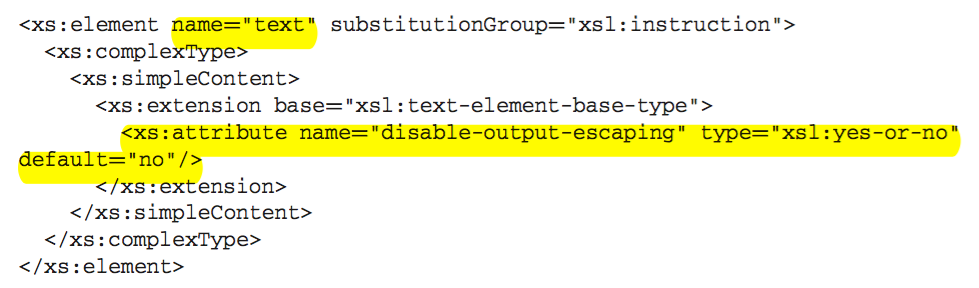
\includegraphics[width=.9\textwidth]{imgs/Schema-text.png}
    \end{center}
    %\textit{In parte già disponibili nei moduli TEI di base}

\end{frame}

\begin{frame}
    \frametitle{Visualizzare ed Elaborare documenti XML}
    \addtocounter{nframe}{1}
    
    %\begin{center}
    %    
\includegraphics[width=.2\textwidth]{../imgs/tei-r.pdf}
    %\end{center}
    %\textit{In parte già disponibili nei moduli TEI di base}

     \begin{block}{Attributi Elemento \texttt{<xsl:text>}}
    %     \emph{Per la critica testuale indispensabili i moduli}
         \begin{itemize}
             \item \textbf{disable-output-escaping}: se "yes", consente di copiare i caratteri di marcatura non identificati nell'albero di output.
        \end{itemize}
     \end{block}
    
\end{frame}

\begin{frame}
    \frametitle{Visualizzare ed Elaborare documenti XML}
    \addtocounter{nframe}{1}
    
    %\begin{center}
    %    
\includegraphics[width=.2\textwidth]{../imgs/tei-r.pdf}
    %\end{center}
    %\textit{In parte già disponibili nei moduli TEI di base}

     \begin{block}{Esempio Elemento \texttt{<xsl:text>}}
        
        \texttt{<xsl:for-each select="\$attr" >}
        \\\texttt{<xsl:value-of select="concat('[',position(),']',current())" />}
        \\\texttt{<xsl:text>&#32;</xsl:text>}
        \\\texttt{</xsl:for-each>}

     \end{block}

\end{frame}

%% if
\begin{frame}
    \frametitle{Visualizzare ed Elaborare documenti XML}
    \addtocounter{nframe}{1}
    
    %\begin{center}
    %    
\includegraphics[width=.2\textwidth]{../imgs/tei-r.pdf}
    %\end{center}
    %\textit{In parte già disponibili nei moduli TEI di base}

     \begin{block}{Elemento \texttt{<xsl:if>}}
        Identifica una condizione semplice: la regola viene eseguita soltanto se la condizione viene soddisfatta.
     \end{block}

\end{frame}

\begin{frame}
    \frametitle{Visualizzare ed Elaborare documenti XML}
    \addtocounter{nframe}{1}
    
    \begin{center}
        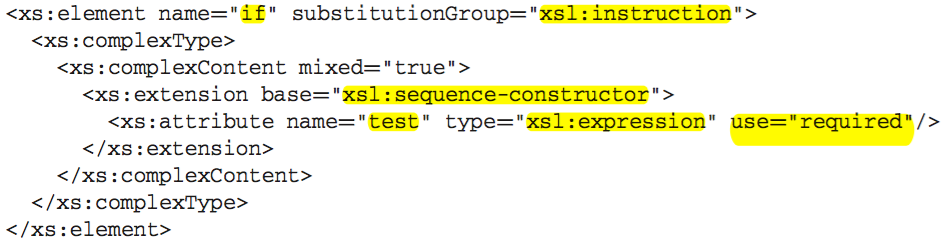
\includegraphics[width=.9\textwidth]{imgs/Schema-if.png}
    \end{center}
    %\textit{In parte già disponibili nei moduli TEI di base}

\end{frame}

\begin{frame}
    \frametitle{Visualizzare ed Elaborare documenti XML}
    \addtocounter{nframe}{1}
    
    %\begin{center}
    %    
\includegraphics[width=.2\textwidth]{../imgs/tei-r.pdf}
    %\end{center}
    %\textit{In parte già disponibili nei moduli TEI di base}

     \begin{block}{Attributi Elemento \texttt{<xsl:if>}}
    %     \emph{Per la critica testuale indispensabili i moduli}
         \begin{itemize}
             \item \textbf{test}: l’espressione di test. Se restituisce true, il contenuto di \texttt{<xsl:if>} viene valutato e inserito nell’albero di output; altrimenti viene ignorato
        \end{itemize}
     \end{block}
    
\end{frame}

\begin{frame}
    \frametitle{Visualizzare ed Elaborare documenti XML}
    \addtocounter{nframe}{1}
    
    %\begin{center}
    %    
\includegraphics[width=.2\textwidth]{../imgs/tei-r.pdf}
    %\end{center}
    %\textit{In parte già disponibili nei moduli TEI di base}

     \begin{block}{Esempio Elemento \texttt{<xsl:if>}}
        
        \texttt{<xsl:if test="@n='23'" >...</xsl:if>}
        \\\texttt{<xsl:if test="title[@level='m']" >...</xsl:if>}
        \\\texttt{<xsl:if test="count(verse) > 3" >...</xsl:if>}
        \\\texttt{}

     \end{block}

\end{frame}


%% xsl:choose
\begin{frame}
    \frametitle{Visualizzare ed Elaborare documenti XML}
    \addtocounter{nframe}{1}
    
    %\begin{center}
    %    
\includegraphics[width=.2\textwidth]{../imgs/tei-r.pdf}
    %\end{center}
    %\textit{In parte già disponibili nei moduli TEI di base}

     \begin{block}{Elemento \texttt{<xsl:choose>}}
        Permette di definire condizioni multiple tra cui scegliere.
     \end{block}

     \begin{block}{Elemento \texttt{<xsl:choose>}}
        Il content model di \textit{choose} prevede uno o più elementi \texttt{<xsl:when>} e opzionalmente l'elemento \texttt{<xsl:otherwise>}.
     \end{block}

\end{frame}

\begin{frame}
    \frametitle{Visualizzare ed Elaborare documenti XML}
    \addtocounter{nframe}{1}
    
    \begin{center}
        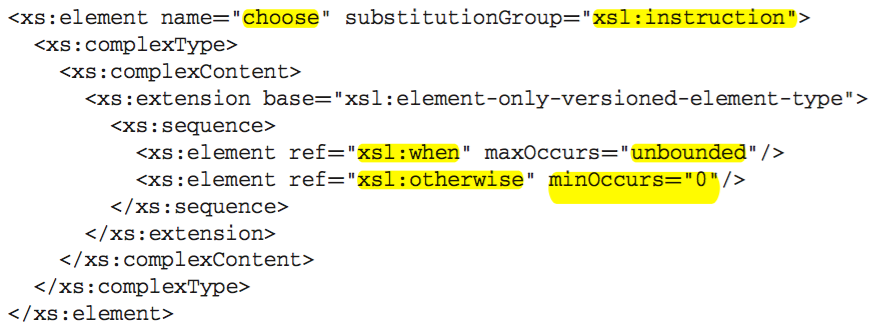
\includegraphics[width=.9\textwidth]{imgs/Schema-choose.png}
    \end{center}
    %\textit{In parte già disponibili nei moduli TEI di base}

\end{frame}

% \begin{frame}
%     \frametitle{Visualizzare ed Elaborare documenti XML}
%     \addtocounter{nframe}{1}
    
%     %\begin{center}
%     %    \includegraphics[width=.2\textwidth]{../imgs/tei-r.pdf}
%     %\end{center}
%     %\textit{In parte già disponibili nei moduli TEI di base}

%      \begin{block}{Attributi Elemento \texttt{<xsl:if>}}
%     %     \emph{Per la critica testuale indispensabili i moduli}
%          \begin{itemize}
%              \item \textbf{test}: l’espressione di test. Se restituisce true, il contenuto di \texttt{<xsl:if>} viene valutato e inserito nell’albero di output; altrimenti viene ignorato
%         \end{itemize}
%      \end{block}
    
% \end{frame}

\begin{frame}
    \frametitle{Visualizzare ed Elaborare documenti XML}
    \addtocounter{nframe}{1}
    
    %\begin{center}
    %    \includegraphics[width=.2\textwidth]{../imgs/tei-r.pdf}
    %\end{center}
    %\textit{In parte già disponibili nei moduli TEI di base}

     \begin{block}{Esempio Elemento \texttt{<xsl:if>}}
        
        \texttt{<xsl:template match="tei:title" >}
        \\\texttt{<xsl:choose>}
        \\\texttt{<xsl:when test="@level = 'm' or @level = 'u'" >}
        \\\texttt{<i><xsl:apply-templates/>. </i> </xsl:when>}
        \\\texttt{<xsl:when test="@level = 'j'" >}
        \\\texttt{<i><xsl:apply-templates/></i>}
        \\\texttt{</xsl:when>}
        \\\texttt{<xsl:otherwise>}
        \\\texttt{<i><xsl:apply-templates/></i></xsl:otherwise>}
        \\\texttt{</xsl:choose></xsl:template>}
     \end{block}

\end{frame}

% xsl:sort

\begin{frame}
    \frametitle{Visualizzare ed Elaborare documenti XML}
    \addtocounter{nframe}{1}
    
    %\begin{center}
    %    \includegraphics[width=.2\textwidth]{../imgs/tei-r.pdf}
    %\end{center}
    %\textit{In parte già disponibili nei moduli TEI di base}

     \begin{block}{Elemento \texttt{<xsl:sort>}}
        Permette di riorganizzare l’ordine in cui vengono scritti i nodi nell’albero di output.
     \end{block}

     \begin{block}{Elemento \texttt{<xsl:sort>}}
        Deve comparire all’interno di un’istruzione \texttt{<xsl:apply-templates>} o \texttt{<xsl:for-each>}.
     \end{block}

\end{frame}

\begin{frame}
    \frametitle{Visualizzare ed Elaborare documenti XML}
    \addtocounter{nframe}{1}
    
    \begin{center}
        \includegraphics[width=.9\textwidth]{imgs/Schema-sort.png}
    \end{center}
    %\textit{In parte già disponibili nei moduli TEI di base}

\end{frame}

\begin{frame}
    \frametitle{Visualizzare ed Elaborare documenti XML}
    \addtocounter{nframe}{1}
    
    %\begin{center}
    %    \includegraphics[width=.2\textwidth]{../imgs/tei-r.pdf}
    %\end{center}
    %\textit{In parte già disponibili nei moduli TEI di base}

     \begin{block}{Attributi Elemento \texttt{<xsl:sort>}}
    %     \emph{Per la critica testuale indispensabili i moduli}
         \begin{itemize}
             \item \textbf{select}: espressione XPath per individuare gli elementi in base ai quali effettuare l’ordinamento.
             \item \textbf{lang}: linguaggio utilizzato per l’ordinamento.
             \item \textbf{data-type}: il tipo degli elementi rispetto ai quali stiamo effettuando l’ordinamento.
             \item \textbf{order}: ordinamento crescente (ascending) o discendente (descending)
             \item \textbf{case-order}: indica se dare precedenza ai caratteri minuscoli (lower-first) o maiuscoli (upper-first)
        \end{itemize}
     \end{block}
    
\end{frame}

\begin{frame}
    \frametitle{Visualizzare ed Elaborare documenti XML}
    \addtocounter{nframe}{1}
    
    %\begin{center}
    %    \includegraphics[width=.2\textwidth]{../imgs/tei-r.pdf}
    %\end{center}
    %\textit{In parte già disponibili nei moduli TEI di base}

     \begin{block}{Esempio Elemento \texttt{<xsl:sort>}}
        
        \texttt{<div><ul><xsl:for-each select="TEI/text/body/div" >}
        \\\texttt{<xsl:sort select="@n" data-type="number" order="descending" />}
        \\\texttt{<li><xsl:value-of select="@n" />}
        \\\texttt{<xsl:text>|</xsl:text>}
        \\\texttt{<xsl:value-of select="current()" /></li>}
        \\\texttt{</xsl:for-each></ul></div>}

     \end{block}
\end{frame}

%% xsl:variable

\begin{frame}
    \frametitle{Visualizzare ed Elaborare documenti XML}
    \addtocounter{nframe}{1}
    
    %\begin{center}
    %    \includegraphics[width=.2\textwidth]{../imgs/tei-r.pdf}
    %\end{center}
    %\textit{In parte già disponibili nei moduli TEI di base}

     \begin{block}{Elemento \texttt{<xsl:variable>}}
        Permette di definire una variabile, ovvero una posizione di memorizzazione denominata in un modo personalizzato, che contiene i risultati di una espressione valutata a runtime.
     \end{block}

     \begin{block}{Elemento \texttt{<xsl:variable>}}
        L’accesso ad una variabile avviene anteponendo il carattere \$ al nome della variabile (es \$unaVariabile).
     \end{block}

\end{frame}

\begin{frame}
    \frametitle{Visualizzare ed Elaborare documenti XML}
    \addtocounter{nframe}{1}
    
    \begin{center}
        \includegraphics[width=.9\textwidth]{imgs/Schema-variable.png}
    \end{center}
    %\textit{In parte già disponibili nei moduli TEI di base}

\end{frame}

\begin{frame}
    \frametitle{Visualizzare ed Elaborare documenti XML}
    \addtocounter{nframe}{1}
    
    %\begin{center}
    %    \includegraphics[width=.2\textwidth]{../imgs/tei-r.pdf}
    %\end{center}
    %\textit{In parte già disponibili nei moduli TEI di base}

     \begin{block}{Attributi Elemento \texttt{<xsl:variable>}}
    %     \emph{Per la critica testuale indispensabili i moduli}
         \begin{itemize}
             \item \textbf{name}: nome della variabile.
             \item \textbf{select}: seleziona il contenuto della variabile, se presente; altrimenti come contenuto viene usato il contenuto dell’istruzione 
        \end{itemize}
     \end{block}
    
\end{frame}

\begin{frame}
    \frametitle{Visualizzare ed Elaborare documenti XML}
    \addtocounter{nframe}{1}
    
    %\begin{center}
    %    \includegraphics[width=.2\textwidth]{../imgs/tei-r.pdf}
    %\end{center}
    %\textit{In parte già disponibili nei moduli TEI di base}
    \textbf{La definizione di variabili può assumere tre distinte forme:}

     \begin{block}{Esempio Elemento \texttt{<xsl:variable>}}
        \begin{itemize}
            \item creazione di una variabile il cui valore è una stringa vuota
            \item creazione di una variabile avente valore definito dall’attributo select
            \item creazione mediante inclusione di contenuto nel corpo dell’elemento
        \end{itemize}
     \end{block}
\end{frame}

\begin{frame}
    \frametitle{Visualizzare ed Elaborare documenti XML}
    \addtocounter{nframe}{1}
    
    %\begin{center}
    %    \includegraphics[width=.2\textwidth]{../imgs/tei-r.pdf}
    %\end{center}
    %\textit{In parte già disponibili nei moduli TEI di base}
    \textbf{La definizione di variabili può assumere tre distinte forme:}

     \begin{block}{Esempio Elemento \texttt{<xsl:variable>}}
        \begin{itemize}
            \item \texttt{<xsl:variable name="myVar" />}
            \item \texttt{<xsl:variable name="myVar" select="150" />}
            \item \texttt{<xsl:variable name="myVar" >}
            \item[] \texttt{<xs:value-of="@n"/>}
            \item[] \texttt{</xsl:variable>}
        \end{itemize}

     \end{block}
\end{frame}

%% xsl:param

\begin{frame}
    \frametitle{Visualizzare ed Elaborare documenti XML}
    \addtocounter{nframe}{1}
    
    %\begin{center}
    %    \includegraphics[width=.2\textwidth]{../imgs/tei-r.pdf}
    %\end{center}
    %\textit{In parte già disponibili nei moduli TEI di base}

     \begin{block}{Elemento \texttt{<xsl:param>}}
        E' simile ad una \texttt{<xsl:variable>}, ma il suo valore può essere modificato in base al modo in cui il template viene chiamato o dal foglio di stile stesso.
     \end{block}

     \begin{block}{Elemento \texttt{<xsl:param>}}
        Può essere inserita come primo figlio di un \texttt{<xsl:template>}
     \end{block}

\end{frame}

\begin{frame}
    \frametitle{Visualizzare ed Elaborare documenti XML}
    \addtocounter{nframe}{1}
    
    \begin{center}
        \includegraphics[width=.9\textwidth]{imgs/Schema-param.png}
    \end{center}
    %\textit{In parte già disponibili nei moduli TEI di base}

\end{frame}

\begin{frame}
    \frametitle{Visualizzare ed Elaborare documenti XML}
    \addtocounter{nframe}{1}
    
    %\begin{center}
    %    \includegraphics[width=.2\textwidth]{../imgs/tei-r.pdf}
    %\end{center}
    %\textit{In parte già disponibili nei moduli TEI di base}

     \begin{block}{Attributi Elemento \texttt{<xsl:param>}}
    %     \emph{Per la critica testuale indispensabili i moduli}
         \begin{itemize}
             \item \textbf{name}: nome della variabile.
             \item \textbf{select}: seleziona il contenuto della variabile, se presente; altrimenti come contenuto viene usato il contenuto dell’istruzione stessa
        \end{itemize}
     \end{block}
    
\end{frame}

\begin{frame}
    \frametitle{Visualizzare ed Elaborare documenti XML}
    \addtocounter{nframe}{1}
    
    %\begin{center}
    %    \includegraphics[width=.2\textwidth]{../imgs/tei-r.pdf}
    %\end{center}
    %\textit{In parte già disponibili nei moduli TEI di base}

     \begin{block}{Esempio Elemento \texttt{<xsl:param>}}
        
        \texttt{<xsl:template name="body" >}
        \\\texttt{<xsl:param name="style" >color:blue</xsl:param>}
        \\\texttt{<div><xsl:attribute name="style" >}
        \\\texttt{<xsl:value-of select="\$style" />}
        \\\texttt{</xsl:attribute>}
        \\\texttt{<xsl:value-of select="." /></div>}
        \\\texttt{</xsl:template>}

     \end{block}
\end{frame}

%% xsl:call-template
\begin{frame}
    \frametitle{Visualizzare ed Elaborare documenti XML}
    \addtocounter{nframe}{1}
    
    %\begin{center}
    %    \includegraphics[width=.2\textwidth]{../imgs/tei-r.pdf}
    %\end{center}
    %\textit{In parte già disponibili nei moduli TEI di base}

     \begin{block}{Elemento \texttt{<xsl:call-template>}}
        Dopo aver assegnato un nome ad un template, è possibile richiamarlo con l’istruzione \texttt{<xsl:call-template>}.
     \end{block}

     \begin{block}{Elemento \texttt{<xsl:call-template>}}
        Per invocare un template passando dei parametri è possibile utilizzare l’elemento \texttt{<xsl:with-param>} nel corpo dell’elemento \texttt{<xsl:call-template>} o \texttt{<xsl:apply-templates>} indicando il nome del parametro ed il valore.
     \end{block}

\end{frame}

\begin{frame}
    \frametitle{Visualizzare ed Elaborare documenti XML}
    \addtocounter{nframe}{1}
    
    \begin{center}
        \includegraphics[width=.9\textwidth]{imgs/Schema-call-template.png}
    \end{center}
    %\textit{In parte già disponibili nei moduli TEI di base}

\end{frame}

\begin{frame}
    \frametitle{Visualizzare ed Elaborare documenti XML}
    \addtocounter{nframe}{1}
    
    %\begin{center}
    %    \includegraphics[width=.2\textwidth]{../imgs/tei-r.pdf}
    %\end{center}
    %\textit{In parte già disponibili nei moduli TEI di base}

     \begin{block}{Attributi Elemento \texttt{<xsl:call-template>}}
    %     \emph{Per la critica testuale indispensabili i moduli}
         \begin{itemize}
             \item \textbf{name}: il nome del template da richiamare. Il foglio di stile deve necessariamente contenere un \texttt{<xsl:template>} con tale nome specificato
        \end{itemize}
     \end{block}
    
\end{frame}

\begin{frame}
    \frametitle{Visualizzare ed Elaborare documenti XML}
    \addtocounter{nframe}{1}
    
    %\begin{center}
    %    \includegraphics[width=.2\textwidth]{../imgs/tei-r.pdf}
    %\end{center}
    %\textit{In parte già disponibili nei moduli TEI di base}

     \begin{block}{Esempio Elemento \texttt{<xsl:call-template>}}
        
        \texttt{<body>}
        \\\texttt{<xsl:call-template name="body" >}
        \\\texttt{<xsl:with-param name="style" >color:red</xsl:with-param>}
        \\\texttt{</xsl:call-template></body>}

     \end{block}
\end{frame}


%% xsl:element
\begin{frame}
    \frametitle{Visualizzare ed Elaborare documenti XML}
    \addtocounter{nframe}{1}
    
    %\begin{center}
    %    \includegraphics[width=.2\textwidth]{../imgs/tei-r.pdf}
    %\end{center}
    %\textit{In parte già disponibili nei moduli TEI di base}

     \begin{block}{Elemento \texttt{<xsl:element>}}
        Per creare elementi è possibile utilizzare l'istruzione \texttt{<xsl:element>}.
     \end{block}

\end{frame}

\begin{frame}
    \frametitle{Visualizzare ed Elaborare documenti XML}
    \addtocounter{nframe}{1}
    
    \begin{center}
        \includegraphics[width=.9\textwidth]{imgs/Schema-element.png}
    \end{center}
    %\textit{In parte già disponibili nei moduli TEI di base}

\end{frame}

\begin{frame}
    \frametitle{Visualizzare ed Elaborare documenti XML}
    \addtocounter{nframe}{1}
    
    \begin{center}
        \includegraphics[width=.9\textwidth]{imgs/element-example.png}
    \end{center}
    %\textit{In parte già disponibili nei moduli TEI di base}

\end{frame}


%% xsl:attribute

\begin{frame}
    \frametitle{Visualizzare ed Elaborare documenti XML}
    \addtocounter{nframe}{1}
    
    %\begin{center}
    %    \includegraphics[width=.2\textwidth]{../imgs/tei-r.pdf}
    %\end{center}
    %\textit{In parte già disponibili nei moduli TEI di base}

     \begin{block}{Elemento \texttt{<xsl:attribute>}}
        E' possibile create attributi utilizzando l’elemento \texttt{<xsl:attribute>} ed indicando negli attributi \textit{name} e \textit{namespace} (opzionale) il nome e il namespace di appartenenza dell’attributo.
     \end{block}

\end{frame}

\begin{frame}
    \frametitle{Visualizzare ed Elaborare documenti XML}
    \addtocounter{nframe}{1}
    
    \begin{center}
        \includegraphics[width=.9\textwidth]{imgs/Schema-attributo.png}
    \end{center}
    %\textit{In parte già disponibili nei moduli TEI di base}

\end{frame}


\begin{frame}
    \frametitle{Visualizzare ed Elaborare documenti XML}
    \addtocounter{nframe}{1}
    
    %\begin{center}
    %    \includegraphics[width=.2\textwidth]{../imgs/tei-r.pdf}
    %\end{center}
    %\textit{In parte già disponibili nei moduli TEI di base}

     \begin{block}{Esempio Elemento \texttt{<xsl:attribute>}}
        
        \texttt{<xsl:element name="div" >}
        \\\texttt{<xsl:attribute name="id" >}
        \\\texttt{<xsl:value-of select="@id"/>}
        \\\texttt{</xsl:attribute>}
        \\\texttt{</xsl:element>}

     \end{block}
\end{frame}


%% xsl:comment
\begin{frame}
    \frametitle{Visualizzare ed Elaborare documenti XML}
    \addtocounter{nframe}{1}
    
    %\begin{center}
    %    \includegraphics[width=.2\textwidth]{../imgs/tei-r.pdf}
    %\end{center}
    %\textit{In parte già disponibili nei moduli TEI di base}

     \begin{block}{Altri Elemento di creazione}
        \begin{itemize}
            \item \textbf{commenti}: mediante \texttt{<xsl:comment>} specificando fra i tag di apertura e chiusura il testo del commento:
            \item[] ...
            \item \textbf{processing instruction}: si utilizza \texttt{<xsl:processing-instruction>} specificando mediante l’attributo name il nome ed inserendone il contenuto tra i tag di apertura e chiusura
            \item[] ...
            \item \textbf{testo}: si usa \texttt{<xsl:text>} specificando nel corpo il contenuto della sezione CDATA.
            \item[] ...  
        \end{itemize}
     \end{block}

\end{frame}

% spazi bianchi
\begin{frame}
    \frametitle{Visualizzare ed Elaborare documenti XML}
    \addtocounter{nframe}{1}
    
    %\begin{center}
    %    \includegraphics[width=.2\textwidth]{../imgs/tei-r.pdf}
    %\end{center}
    %\textit{In parte già disponibili nei moduli TEI di base}

     \begin{block}{Gestione spazi bianchi}
        La gestione degli spazi bianchi nel documento di origine è specificato dalle regole di scarto attraverso le istruzioni \textbf{xsl:preserve-space} e \textbf{xsl:strip-space}.
     \end{block}

\end{frame}


%% xsl:preserve-space
\begin{frame}
    \frametitle{Visualizzare ed Elaborare documenti XML}
    \addtocounter{nframe}{1}
    
    %\begin{center}
    %    \includegraphics[width=.2\textwidth]{../imgs/tei-r.pdf}
    %\end{center}
    %\textit{In parte già disponibili nei moduli TEI di base}

     \begin{block}{Elemento \texttt{<xsl:preserve-space>}}
         Elenca gli elementi dell'albero di origine in cui devono essere conservati gli spazi bianchi originali.
     \end{block}

     \begin{block}{Esempio \texttt{<xsl:preserve-space>}}
        \texttt{<xsl:preserve-space elements="p head"/>}
    \end{block}

\end{frame}

\begin{frame}
    \frametitle{Visualizzare ed Elaborare documenti XML}
    \addtocounter{nframe}{1}
    
    \begin{center}
        \includegraphics[width=.9\textwidth]{imgs/Schema-preserve-space.png}
    \end{center}

\end{frame}

%%  xsl:strip-space

\begin{frame}
    \frametitle{Visualizzare ed Elaborare documenti XML}
    \addtocounter{nframe}{1}
    
    %\begin{center}
    %    \includegraphics[width=.2\textwidth]{../imgs/tei-r.pdf}
    %\end{center}
    %\textit{In parte già disponibili nei moduli TEI di base}

     \begin{block}{Elemento \texttt{<xsl:strip-space>}}
        Elenca gli elementi dell'albero di origine in cui devono essere scartati gli spazi bianchi originali
     \end{block}

     \begin{block}{Esempio \texttt{<xsl:strip-space>}}
       \texttt{ <xsl:strip-space elements = "*"/>}
     \end{block}

\end{frame}

\begin{frame}
    \frametitle{Visualizzare ed Elaborare documenti XML}
    \addtocounter{nframe}{1}
    
    \begin{center}
        \includegraphics[width=.9\textwidth]{imgs/Schema-strip-space.png}
    \end{center}

\end{frame}

\begin{frame}
    \frametitle{Visualizzare ed Elaborare documenti XML}
    \addtocounter{nframe}{1}
    
    \begin{block}{Esercizio}
        Modificare opportunamente il file template.xsl aggiungendo variabili, parametri e call template.
    \end{block}

\end{frame}



    
    \section{XPath: selezione dei nodi ed espression axes}
    % \begin{frame}
%     \frametitle{Visualizzare ed Elaborare documenti XML}
%     \addtocounter{nframe}{1}
    
%     %\begin{center}
%     %    \includegraphics[width=.2\textwidth]{../imgs/tei-r.pdf}
%     %\end{center}
%     %\textit{In parte già disponibili nei moduli TEI di base}

%      \begin{block}{Perché visualizzare il testo}
%     %     \emph{Per la critica testuale indispensabili i moduli}
%          \begin{itemize}
%             \item  Controllare la codifica e correggere i refusi
%              \item Assicurarsi che tutto sia stato trascritto correttamente
%              \item Mostrare il testo a persone che non conoscono XML-TEI
%              \item Disporre di una versione del lavoro fuibile
%         \end{itemize}
%      \end{block}
    
% \end{frame}

% \begin{frame}
%     \frametitle{Visualizzare ed Elaborare documenti XML}
%     \addtocounter{nframe}{1}
    
%     \begin{center}
%         \includegraphics[width=.9\textwidth]{imgs/SchemaXSLTprocessing.png}
%     \end{center}
%     %\textit{In parte già disponibili nei moduli TEI di base}

% \end{frame}

\begin{frame}
    \frametitle{Visualizzare ed Elaborare documenti XML}
    \addtocounter{nframe}{1}
    
    %\begin{center}
    %    \includegraphics[width=.2\textwidth]{../imgs/tei-r.pdf}
    %\end{center}
    %\textit{In parte già disponibili nei moduli TEI di base}

    \begin{block}{XPath}
        
        XPath è un \textit{expression language} fondamentale per realizzare fogli di stile XSLT.
        
    \end{block}
     
    \begin{block}{XPath}
        \begin{itemize}
            \item Selezionare nodi in un documento XML
            \item Fare match nell'albero source per selezionare il corretto template
            \item Manipolare dati attraverso funzioni
        \end{itemize}
    \end{block}
    
\end{frame}

\begin{frame}
    \frametitle{Visualizzare ed Elaborare documenti XML}
    \addtocounter{nframe}{1}
    
    %\begin{center}
    %    \includegraphics[width=.2\textwidth]{../imgs/tei-r.pdf}
    %\end{center}
    %\textit{In parte già disponibili nei moduli TEI di base}

    \begin{block}{XPath}
        XPath offre una sintassi estesa (piuttosto verbosa) e una sintassi abbreviata.
    \end{block}

    \begin{block}{XPath}
        Le espressioni XPath permettono di selezionare con grande precisione elementi, attributi, ecc.
    \end{block}
    
\end{frame}

\begin{frame}
    \frametitle{Visualizzare ed Elaborare documenti XML}
    \addtocounter{nframe}{1}
    
    %\begin{center}
    %    \includegraphics[width=.2\textwidth]{../imgs/tei-r.pdf}
    %\end{center}
    %\textit{In parte già disponibili nei moduli TEI di base}

    \begin{block}{Esempi XPath selezione con match}
        \emph{Selezionare \textit{documento XML} oppure tutti i nodi \texttt{<quote>}}
        \begin{itemize}
            \item \texttt{<xsl:template match="/" >}
            \item \texttt{<xsl:template match="quote" >}
        \end{itemize}
        
    \end{block}
     
\end{frame}

\begin{frame}
    \frametitle{Visualizzare ed Elaborare documenti XML}
    \addtocounter{nframe}{1}
    
    %\begin{center}
    %    \includegraphics[width=.2\textwidth]{../imgs/tei-r.pdf}
    %\end{center}
    %\textit{In parte già disponibili nei moduli TEI di base}
 
    \begin{block}{Esempi XPath selezione con match}
        \emph{Per selezionare i nodi \texttt{<title>} "figli", "nipoti" o comunque discendenti di \texttt{<quote>}}
        \begin{itemize}
            \item \texttt{match="quote/title"} \textit{(discendente diretto - figlio)}
            \item \texttt{match="quote/*/title"} \textit{(discendente di secondo livello - nipote)}
            \item \texttt{match="quote//title"} \textit{(discendente a qualsiasi livello)}
        \end{itemize}     
    \end{block}
    
\end{frame}

\begin{frame}
    \frametitle{Visualizzare ed Elaborare documenti XML}
    \addtocounter{nframe}{1}
    
    %\begin{center}
    %    \includegraphics[width=.2\textwidth]{../imgs/tei-r.pdf}
    %\end{center}
    %\textit{In parte già disponibili nei moduli TEI di base}

    \begin{block}{Esempi XPath selezione con match}
        \emph{Per selezionare i nodi \texttt{<quote>} con attributo \texttt{@type} (e valore \textit{book})}
        \begin{itemize}
            \item \texttt{match="quote[@type]"}
            \item \texttt{match="quote[@type='book']"}
        \end{itemize}
        
    \end{block}
    
\end{frame}


\begin{frame}
    \frametitle{Visualizzare ed Elaborare documenti XML}
    \addtocounter{nframe}{1}
    
    %\begin{center}
    %    \includegraphics[width=.2\textwidth]{../imgs/tei-r.pdf}
    %\end{center}
    %\textit{In parte già disponibili nei moduli TEI di base}

    \begin{block}{Esempi XPath selezione con match}
        \emph{Per selezionare i nodi usando il carattere "jolly"}
        \begin{itemize}
            \item \texttt{match="*"}
            \item \texttt{match="*[@type]"}
            \item \texttt{match="*[@type='book']"}
        \end{itemize}
    \end{block}
    
\end{frame}


\begin{frame}
    \frametitle{Visualizzare ed Elaborare documenti XML}
    \addtocounter{nframe}{1}
    
    %\begin{center}
    %    \includegraphics[width=.2\textwidth]{../imgs/tei-r.pdf}
    %\end{center}
    %\textit{In parte già disponibili nei moduli TEI di base}

    \begin{block}{Esempi XPath selezione con match}
        \emph{Per selezionare più di un elemento (operatore OR) oppure per selezionare un nodo con uno specifico ID}
        \begin{itemize}
            \item \texttt{match="title | author"}
            \item \texttt{match="id('stella-2007')"}
        \end{itemize}
        
    \end{block}
    
\end{frame}

% selezione nodi con select

\begin{frame}
    \frametitle{Visualizzare ed Elaborare documenti XML}
    \addtocounter{nframe}{1}
    
    %\begin{center}
    %    \includegraphics[width=.2\textwidth]{../imgs/tei-r.pdf}
    %\end{center}
    %\textit{In parte già disponibili nei moduli TEI di base}

    \begin{block}{XPath selezione con select}
        Il valore di questo attributo è un'espressione conforme al linguaggio XPath
    \end{block}

    \begin{block}{XPath selezione con select}
        L'attributo select può ricorrere a una sintassi più complessa rispetto a match
    \end{block}
    
\end{frame}

\begin{frame}
    \frametitle{Visualizzare ed Elaborare documenti XML}
    \addtocounter{nframe}{1}
    
    %\begin{center}
    %    \includegraphics[width=.2\textwidth]{../imgs/tei-r.pdf}
    %\end{center}
    %\textit{In parte già disponibili nei moduli TEI di base}

    \begin{block}{L’attributo select è usato con le istruzioni XSLT}
        \begin{itemize}
            \item xsl:apply-templates
            \item xsl:value-of
            \item xsl:copy-of
            \item xsl:for-each
            \item xsl:sort
            \item xsl:variable
            \item xsl:param
        \end{itemize}
    \end{block}

\end{frame}

\begin{frame}
    \frametitle{Visualizzare ed Elaborare documenti XML}
    \addtocounter{nframe}{1}
    
    %\begin{center}
    %    \includegraphics[width=.2\textwidth]{../imgs/tei-r.pdf}
    %\end{center}
    %\textit{In parte già disponibili nei moduli TEI di base}

    \begin{block}{XPath}
        Le espressioni XPath permettono di "navigare" l'albero del documento XML usando assi di navigazione (\textit{expression axes}).
    \end{block}

    \begin{block}{XPath}
        La selezione può essere assoluta o relativa al \textbf{nodo corrente} e si compone di tre parti: (\textbf{Asse}, \textbf{Test}, \textbf{Predicato})
    \end{block}
    
\end{frame}

\begin{frame}
    \frametitle{Visualizzare ed Elaborare documenti XML}
    \addtocounter{nframe}{1}
    
    \begin{center}
        \includegraphics[width=.9\textwidth]{imgs/SchemaAssi-Xpath.png}
    \end{center}

\end{frame}

\begin{frame}
    \frametitle{Visualizzare ed Elaborare documenti XML}
    \addtocounter{nframe}{1}
    
    \begin{center}
        \includegraphics[width=.95\textwidth]{imgs/Schema-Assi-1.png}
    \end{center}

\end{frame}

\begin{frame}
    \frametitle{Visualizzare ed Elaborare documenti XML}
    \addtocounter{nframe}{1}
    
    \begin{center}
        \includegraphics[width=.95\textwidth]{imgs/Schema-Assi-2.png}
    \end{center}

\end{frame}



\begin{frame}
    \frametitle{Visualizzare ed Elaborare documenti XML}
    \addtocounter{nframe}{1}
    
    \begin{center}
        \includegraphics[width=.95\textwidth]{imgs/Sintassi-Abbreviata.png}
    \end{center}

\end{frame}


\begin{frame}
    \frametitle{Visualizzare ed Elaborare documenti XML}
    \addtocounter{nframe}{1}
    
    \begin{center}
        \includegraphics[width=.95\textwidth]{imgs/Sintassi-Abbreviata-Estesa.png}
    \end{center}

\end{frame}


\begin{frame}
    \frametitle{Visualizzare ed Elaborare documenti XML}
    \addtocounter{nframe}{1}
    
    \begin{center}
        \includegraphics[width=.95\textwidth]{imgs/Tab-Operatori-Predicato.png}
    \end{center}

\end{frame}

\begin{frame}
    \frametitle{Visualizzare ed Elaborare documenti XML}
    \addtocounter{nframe}{1}
    
    %\begin{center}
    %    \includegraphics[width=.2\textwidth]{../imgs/tei-r.pdf}
    %\end{center}
    %\textit{In parte già disponibili nei moduli TEI di base}

    \begin{block}{Esempio sintassi estesa - sintassi abbreviata}
        \begin{itemize}
            \item \texttt{<xsl:value-of select="child::author"/>}
            \item \texttt{<xsl:value-of select="author"/>}
        \end{itemize}
    \end{block}

\end{frame}

\begin{frame}
    \frametitle{Visualizzare ed Elaborare documenti XML}
    \addtocounter{nframe}{1}
    
    %\begin{center}
    %    \includegraphics[width=.2\textwidth]{../imgs/tei-r.pdf}
    %\end{center}
    %\textit{In parte già disponibili nei moduli TEI di base}

    \begin{block}{Esempio sintassi estesa - sintassi abbreviata}
        \begin{itemize}
            \item \texttt{<xsl:value-of select="parent::quote"/>}
            \item \texttt{<xsl:value-of select="ancestor::quote"/>}
            \item \texttt{<xsl:value-of select=".."/>}
        \end{itemize}
    \end{block}

\end{frame}

\begin{frame}
    \frametitle{Visualizzare ed Elaborare documenti XML}
    \addtocounter{nframe}{1}
    
    %\begin{center}
    %    \includegraphics[width=.2\textwidth]{../imgs/tei-r.pdf}
    %\end{center}
    %\textit{In parte già disponibili nei moduli TEI di base}

    \begin{block}{Esempio predicati}
        \begin{itemize}
            \item \texttt{//div[@type='chapter']}
            \item \texttt{//div[@type!='chapter']}
            \item \texttt{//div[@n > 2]}
            \item \texttt{//div[1]}
            \item \texttt{//div[last()]}
            \item \texttt{//div[position() = last() - 1]}
            \item \texttt{//div[position() mod 2 = 0]}
        \end{itemize}
    \end{block}

\end{frame}


    
    \section{Conclusioni}
    % \begin{frame}
%     \frametitle{Visualizzare ed Elaborare documenti XML}
%     \addtocounter{nframe}{1}
    
%     %\begin{center}
%     %    \includegraphics[width=.2\textwidth]{../imgs/tei-r.pdf}
%     %\end{center}
%     %\textit{In parte già disponibili nei moduli TEI di base}

%      \begin{block}{Perché visualizzare il testo}
%     %     \emph{Per la critica testuale indispensabili i moduli}
%          \begin{itemize}
%             \item  Controllare la codifica e correggere i refusi
%              \item Assicurarsi che tutto sia stato trascritto correttamente
%              \item Mostrare il testo a persone che non conoscono XML-TEI
%              \item Disporre di una versione del lavoro fuibile
%         \end{itemize}
%      \end{block}
    
% \end{frame}

% \begin{frame}
%     \frametitle{Visualizzare ed Elaborare documenti XML}
%     \addtocounter{nframe}{1}
    
%     \begin{center}
%         \includegraphics[width=.9\textwidth]{imgs/SchemaXSLTprocessing.png}
%     \end{center}
%     %\textit{In parte già disponibili nei moduli TEI di base}

% \end{frame}

% Controllo e gestione degli spazi bianchi p 54 slide di Chiara

\begin{frame}
    \frametitle{Visualizzare ed Elaborare documenti XML}
    \addtocounter{nframe}{1}
    
    %\begin{center}
    %    \includegraphics[width=.2\textwidth]{../imgs/tei-r.pdf}
    %\end{center}
    %\textit{In parte già disponibili nei moduli TEI di base}

     \begin{block}{XSLT: come procedere per un buon risultato}
    %     \emph{Per la critica testuale indispensabili i moduli}
         \begin{itemize}
            \item Tracciare una mappa della conversione da XML a (X)HTML
             \item Lasciare il \texttt{<teiHeader>} per ultimo
             \item Definire lo scheletro HTML sul primo \textbf{template rule} e controllare che funzioni
        \end{itemize}
     \end{block}
    
\end{frame}

\begin{frame}
    \frametitle{Visualizzare ed Elaborare documenti XML}
    \addtocounter{nframe}{1}
    
    %\begin{center}
    %    \includegraphics[width=.2\textwidth]{../imgs/tei-r.pdf}
    %\end{center}
    %\textit{In parte già disponibili nei moduli TEI di base}

     \begin{block}{XSLT: come procedere per un buon risultato}
    %     \emph{Per la critica testuale indispensabili i moduli}
         \begin{itemize}
             \item Divisione strutturale: uso di intestazioni (\texttt{<h1>, <h2> ecc.}) e
             paragrafi, a capo (\texttt{<p>, <br/>}) in HTML
             \item Formattazione degli elementi: usate gli elementi già presenti in
             HTML (\texttt{<b>, <i>, ecc.}) oppure definite degli \texttt{<span>}.
             \item Scrivere una regola alla volta, testarla e solo se funziona passare alla
             successiva
        \end{itemize}
     \end{block}
    
\end{frame}


\begin{frame}
    \frametitle{Visualizzare ed Elaborare documenti XML}
    \addtocounter{nframe}{1}
    
    %\begin{center}
    %    \includegraphics[width=.2\textwidth]{../imgs/tei-r.pdf}
    %\end{center}
    %\textit{In parte già disponibili nei moduli TEI di base}

     \begin{block}{XSLT: come procedere per XML-TEI}
        Tutti i nomi di elementi TEI devono essere preceduti dal prefisso \textbf{tei:}!
     \end{block}

     \begin{block}{XSLT: come procedere per XML-TEI}
        \texttt{<xsl:stylesheet version="1.0"}
        \\\texttt{ xmlns:xsl="http://www.w3.org/1999/XSL/Transform"}
        \\\texttt{ xmlns:tei="http://www.tei-c.org/ns/1.0"}
        \\\texttt{ xmlns="http://www.w3.org/1999/xhtml" >}
     \end{block}
    
\end{frame}

   

\begin{frame}
    \frametitle{Visualizzare ed Elaborare documenti XML}
    \addtocounter{nframe}{1}
    
    %\begin{center}
    %    \includegraphics[width=.2\textwidth]{../imgs/tei-r.pdf}
    %\end{center}
    %\textit{In parte già disponibili nei moduli TEI di base}

     \begin{block}{Fogli di stile TEI}
        Gli sviluppatori della TEI mettono a disposizione dei fogli di stile per documenti TEI P4 e posteriori
        \\\texttt{http://www.tei-c.org/Tools/Stylesheets/}
     \end{block}

     \begin{block}{XSLT per XML-TEI}
        \texttt{http://sourceforge.net/projects/tei/}
        \\\texttt{http://tei.oucs.ox.ac.uk/teideb/binary}
        \\\texttt{http://www.tei-c.org/oxgarage/}
        \\\texttt{http://wiki.tei-c.org/index.php/Stylesheets}
        \\\texttt{git hub TEI/TEIC}
     \end{block}
    
\end{frame}


\begin{frame}
    \frametitle{Visualizzare ed Elaborare documenti XML}
    \addtocounter{nframe}{1}
    
    %\begin{center}
    %    \includegraphics[width=.2\textwidth]{../imgs/tei-r.pdf}
    %\end{center}
    %\textit{In parte già disponibili nei moduli TEI di base}

     \begin{block}{Riferimenti}
            \begin{itemize}
                \item Michael Kay, XSLT 2.0 and XPath 2.0 Programmer's Reference
                \item James Clark, XSL Transformations (XSLT) Version 1.0, W3C Recommendation 16 November 1999, http://www.w3.org/TR/xslt
                \item E.R. Harold, XSL Transformations (XSLT), capitolo 14 del libro XML
                Bible, disponibile in rete:
                \item[] \url{http://metalab.unc.edu/xml/books/bible/updates/14.html} 
            \end{itemize}
     \end{block}
    
\end{frame}



    
    \end{document}